\documentclass[a4]{article}

% PACKAGES %%%%%%%%%%%%%%%%%%%%%%%%%%%%%%%%%%%%%%%%%%%%%%%%%%%%%%%%%%%%%%%%%%%%%
\usepackage[utf8]{inputenc}
\usepackage{framed}
\usepackage{makecell}
\usepackage[english]{babel}

\usepackage{url}

%!TEX encoding = UTF-8 Unicode

\setlength{\textwidth}{6.5 in}
\setlength{\textheight}{8.5 in}
\setlength{\headsep}{0.5 in}

\usepackage{multirow, array}
\usepackage{float}
\usepackage{charter}

\usepackage[breaklinks=true]{hyperref}

\usepackage{amsmath,longtable,siunitx, float, graphicx, dcolumn, bm, fancyhdr, subcaption, caption, multicol, setspace}
\usepackage{amssymb}

\usepackage[hmarginratio=1:1, top=32mm, columnsep=20pt, headsep=\dimexpr20mm, margin=0.8in, top=1in ]{geometry}

\usepackage{booktabs}
\usepackage{enumitem}
\usepackage{tabularx}
\usepackage[table]{xcolor} % [table] provides \cellcolor (loads colortbl)

\usepackage{tikz}
\usetikzlibrary{shapes.geometric, arrows.meta, positioning}

% ----------- global tikz styles (matches the CV challenge docs) -----------
\tikzset{
  font=\scriptsize,
  every node/.style       = {transform shape},
  startstop/.style        = {ellipse, draw, fill=blue!10,
                             inner sep=2pt, minimum width=16mm, align=center},
  process/.style          = {rectangle, draw, fill=orange!15,
                             text width=24mm, inner sep=3pt, align=center},
  data/.style             = {rectangle, draw, fill=green!12, rounded corners,
                             text width=24mm, inner sep=3pt, align=center},
  arrow/.style            = {->, >=Stealth, shorten >=1pt, shorten <=1pt}
}

% Colours for the schedule
\definecolor{heavyweek}{HTML}{FFE8CC}
\definecolor{phase0}{HTML}{D9E8FB}
\definecolor{phase1}{HTML}{DDF4DD}
\definecolor{phase2}{HTML}{F3DDF4}
\definecolor{bufferc}{HTML}{EFEFEF}

\newcommand{\TODO}{\textbf{\textcolor{red}{TODO}}}
\newcommand{\deliv}[1]{\textit{\textbf{Deliverable:} #1}}

\renewcommand{\thesection}{\Roman{section}}

% ----------- header / footer (logos optional, guarded) -----------
\pagestyle{fancy}
\fancyhf{}
\lhead{\IfFileExists{CETC.png}{\includegraphics[scale=0.4]{CETC.png}}{\small\textbf{CETC}}}
\rhead{\IfFileExists{Cornell-University-Logo.png}{\includegraphics[scale=0.025]{Cornell-University-Logo.png}}{\small Cornell University}}
\cfoot{\thepage}
\renewcommand{\headrulewidth}{0.4pt}
\renewcommand{\footrulewidth}{0pt}

\begin{document}

\thispagestyle{fancy}

\begin{center}
    \textbf{\large Orbit Odyssey -- Natural Language Processing} \\
    {Week-by-Week Project Plan}

    \vspace{0.7em}

    David Alejandro Fuquen \\

    {\small Planning horizon: 21 September 2025 -- 15 November 2025} \\
    {\small \today}
\end{center}

\vspace{0.5em}

% =====================================================================
\section{Overview and Objectives}

The NLP challenge extends the Orbit Odyssey learning arc from computer vision
into language. Following the same space-exploration narrative, students learn
how a machine turns human (and non-human) language into concrete robot actions.
The challenge is delivered in two phases:

\begin{itemize}[leftmargin=*]
    \item \textbf{Phase 1 -- English.} Students read a ``mission log'' written in
    casual astronaut English and teach a small model to convert it into a list of
    robot commands (\texttt{MOVE~2}, \texttt{TURN~90}, \ldots). This establishes
    the full NLP pipeline: tokenization, intent classification, slot extraction,
    and mapping to commands.
    \item \textbf{Phase 2 -- Alien language.} Stranded in space, the crew receives
    a distress transmission in an \emph{unknown alien language}, accompanied by a
    partial ``Rosetta Stone.'' Students reuse the \emph{same} pipeline to decipher
    the message and extract the commands it encodes.
\end{itemize}

\noindent\textbf{Core pedagogical goal.} Using a language nobody in the room
speaks makes the central lesson unavoidable: the model never ``understands''
words like \emph{move} or \emph{forward}. It tokenizes, learns statistical
patterns, and maps them to outputs via the Rosetta correspondence --- exactly as
it did in English, where the illusion of understanding is strongest.

\noindent\textbf{Final artefact of both phases.} A \emph{list of robot commands}
extracted from the message. That list is the boundary of this project (see
\S\ref{sec:decisions}); actually driving the physical XRP robot is out of scope.

% =====================================================================
\section{Locked Design Decisions}\label{sec:decisions}

The following were agreed during planning and frame every task below.

\begin{center}
\renewcommand{\arraystretch}{1.3}
\begin{tabularx}{\linewidth}{@{}p{3.4cm}X@{}}
\toprule
\textbf{Decision} & \textbf{Resolution} \\
\midrule
Web platform &
Rebuild the current Streamlit prototype as a \textbf{standalone Next.js web
application} (browser-accessible, no local Python install for students). \\

NLP approach &
A \textbf{small, genuinely trainable intent~+~slot model} that students train
themselves --- mirroring the ``train your own model'' arc of the CV challenge,
rather than a hand-written rule table. \\

Robot execution &
\textbf{Out of scope.} The deliverable is the extracted \emph{command list}
that \emph{would} be handed to the XRP. No serial/hardware integration. \\

Alien language &
A \textbf{fixed constructed mini-grammar} (novel vocabulary, distinct word
order/morphology) with a \textbf{partial Rosetta Stone}, and
\textbf{per-session relexification} (swap surface word-forms per team) for
replayability and anti-cheat. \\
\bottomrule
\end{tabularx}
\end{center}

% =====================================================================
\section{System Architecture}

\subsection*{Target stack}
\begin{itemize}[leftmargin=*]
    \item \textbf{Next.js (App Router)} single application: student-facing UI plus
    lightweight API routes for content, seeds, and answer-key checks.
    \item \textbf{In-browser training with TensorFlow.js} as the recommended model
    runtime: students watch loss/accuracy update live (echoing the CV challenge's
    WebSocket progress), and no GPU server is required. \emph{Fallback:} a small
    Python/FastAPI training microservice if a heavier model proves necessary
    (open question, \S\ref{sec:open}).
    \item \textbf{Domain logic in TypeScript}, ported from the Streamlit prototype:
    tokenizer, command grammar, and the existing 2D path simulator (reused only as
    an optional auto-grader, not for robot control).
\end{itemize}

\subsection*{The model (shared across both phases)}
\begin{itemize}[leftmargin=*]
    \item \textbf{Intent classifier}: per clause, predict the action
    (\texttt{MOVE} / \texttt{TURN}; optionally \texttt{STOP} later).
    \item \textbf{Slot extractor}: token-level tagging for the numeric amount and
    direction (e.g.\ tiles, degrees, left/right), assembled into the final command.
    \item \textbf{Training data}: an authored, augmented parallel corpus
    (sentence $\rightarrow$ command). In Phase 2 the \emph{same} architecture is
    retrained on the Rosetta correspondence over alien tokens.
\end{itemize}

\subsection*{Pipeline}
\begin{center}
\begin{tikzpicture}[node distance=6mm and 9mm]
  \node[data]     (msg)   {Mission log / \\ alien message};
  \node[process]  (tok)   [right=of msg]  {Tokenize};
  \node[process]  (intent)[right=of tok]  {Intent \\ classify};
  \node[process]  (slot)  [right=of intent]{Slot \\ extract};
  \node[startstop](cmd)   [right=of slot]  {Command \\ list};
  \draw[arrow] (msg)--(tok);
  \draw[arrow] (tok)--(intent);
  \draw[arrow] (intent)--(slot);
  \draw[arrow] (slot)--(cmd);
  \node[data] (rosetta) [below=8mm of intent] {Training data / \\ Rosetta Stone};
  \draw[arrow] (rosetta) -- (intent);
  \draw[arrow] (rosetta) -| (slot);
\end{tikzpicture}
\end{center}

% =====================================================================
\section{Phase Map}

\begin{center}
\renewcommand{\arraystretch}{1.3}
\begin{tabularx}{\linewidth}{@{}p{3.2cm}p{3.4cm}X@{}}
\toprule
\textbf{Phase} & \textbf{Weeks} & \textbf{Outcome} \\
\midrule
\cellcolor{phase0}Phase 0 -- Migration &
Wk 1 (Sep 21--27) &
Streamlit prototype rebuilt as a navigable Next.js app; domain logic ported. \\

\cellcolor{phase1}Phase 1 -- English &
Wk 2--3 (Sep 28--Oct 11) &
Trainable intent+slot model; students decode English logs into command lists. \\

\cellcolor{phase2}Phase 2 -- Alien &
Wk 4--6 (Oct 12--Nov 1) &
Constructed language, Rosetta Stone, and deciphering flow reusing the model. \\

\cellcolor{bufferc}Hardening &
Wk 7--8 (Nov 2--15) &
Documentation, scoring, pilot testing, deployment, and buffer. \\
\bottomrule
\end{tabularx}
\end{center}

% =====================================================================
\section{Week-by-Week Schedule}

\begin{center}
\renewcommand{\arraystretch}{1.35}
\begin{tabularx}{\linewidth}{@{}p{1.1cm}p{2.6cm}X@{}}
\toprule
\textbf{Wk} & \textbf{Dates} & \textbf{Focus \& primary deliverable} \\
\midrule
\cellcolor{phase0}1 & Sep 21--27 & Migration kickoff: Next.js scaffold, ported logic, dataset schema. \\
\cellcolor{heavyweek}\textbf{2} & \textbf{Sep 28--Oct 4} & \textbf{HEAVY WEEK.} Build the trainable English intent+slot model, live-training UI, corpus, end-to-end decode. \\
\cellcolor{phase1}3 & Oct 5--11 & Finalize \& formalize the English phase; scoring; first Student Guide draft. \\
\cellcolor{phase2}4 & Oct 12--18 & Design the alien mini-grammar, generator, relexification, and Rosetta Stone. \\
\cellcolor{phase2}5 & Oct 19--25 & Integrate the alien phase into the shared pipeline (decipher $\rightarrow$ commands). \\
\cellcolor{phase2}6 & Oct 26--Nov 1 & Scoring, moderator tooling, per-team seeds, anti-cheat, command-list export. \\
\cellcolor{bufferc}7 & Nov 2--8 & Documentation (Student/Moderator guides), content polish, pilot test, bug fixing. \\
\cellcolor{bufferc}8 & Nov 9--15 & Final hardening, deployment, QA, content freeze, buffer, handoff. \\
\bottomrule
\end{tabularx}
\end{center}

\noindent The week of \textbf{28 September--4 October} is the maximum-availability
window, so the highest-risk, highest-effort work (the trainable model and the
full end-to-end English loop) is deliberately concentrated there.

\subsection*{Week 1 --- Sep 21--27 \quad (Phase 0: Migration)}
\emph{Moderate availability. Goal: a running Next.js skeleton and clean foundations.}
\begin{itemize}[leftmargin=*, itemsep=1pt]
    \item Initialize the Next.js project, repository, tooling, and CI/lint basics.
    \item Recreate the six-step flow from the Streamlit prototype as navigable
    Next.js routes/pages (static shell, no model yet): Read Log $\rightarrow$
    Extract $\rightarrow$ Translate $\rightarrow$ Train/Dictionary $\rightarrow$
    Decode New Log $\rightarrow$ Compare.
    \item Port domain logic to TypeScript: tokenizer, command grammar
    (\texttt{MOVE}/\texttt{TURN}), and the 2D path simulator (as optional grader).
    \item Choose and spike the model runtime (TensorFlow.js in-browser) with a
    ``hello-world'' train loop to de-risk Week 2.
    \item Draft the English labeled-dataset schema (sentence $\rightarrow$ command).
\end{itemize}
\deliv{Navigable Next.js app skeleton; ported simulator/tokenizer; TF.js training spike; dataset schema.}

\subsection*{Week 2 --- Sep 28--Oct 4 \quad (Phase 1: English core) \hfill \textcolor{orange!80!black}{\textbf{[HEAVY WEEK]}}}
\emph{Maximum availability. Goal: the English challenge works end to end.}
\begin{itemize}[leftmargin=*, itemsep=1pt]
    \item Implement the trainable \textbf{intent classifier} and \textbf{slot
    extractor} in TF.js (tokenizer $\rightarrow$ embedding $\rightarrow$
    intent~+~slot heads).
    \item Build the \textbf{training UI}: label examples, start training, and watch
    loss/accuracy update live.
    \item Author and augment the \textbf{English training corpus} (synonyms,
    numbers, quarter/half turns) plus a held-out ``new mission log'' test set.
    \item Wire \textbf{prediction $\rightarrow$ command list}, and connect the path
    simulator as an optional ``did your commands land correctly?'' auto-grader.
    \item First full playthrough of Phase 1 by the author.
\end{itemize}
\deliv{End-to-end English phase: student labels data, trains the model, decodes a new log into a command list, and sees results.}

\subsection*{Week 3 --- Oct 5--11 \quad (Phase 1: finalize \& formalize)}
\begin{itemize}[leftmargin=*, itemsep=1pt]
    \item Polish UX and the ``reveal'' framing (tokenization vs.\ understanding).
    \item Define the \textbf{scoring rubric} for Phase 1 (command correctness,
    optional path distance) and reference answers.
    \item Add teacher/moderator controls (edit logs, seed corpus, view answer key).
    \item Handle edge cases (unknown words, missing numbers, ambiguous turns).
    \item Draft the \textbf{Student Guide (English phase)} in LaTeX, matching the CV
    challenge document style.
\end{itemize}
\deliv{English phase feature-complete, scored, and documented (draft guide).}

\subsection*{Week 4 --- Oct 12--18 \quad (Phase 2: alien language design)}
\begin{itemize}[leftmargin=*, itemsep=1pt]
    \item Design the \textbf{fixed mini-grammar}: a $\sim$30--60 word lexicon,
    word order (e.g.\ verb-final), and morphology encoding amount/direction
    (gSCAN-inspired command grammar).
    \item Build the \textbf{generator} that emits a distress message, its command
    ground-truth, and a \textbf{partial Rosetta Stone} (enough to deduce most --- not
    all --- rules).
    \item Implement \textbf{relexification}: a per-team seed swaps surface
    word-forms while keeping the grammar fixed.
    \item Validate \textbf{solvability} by hand: confirm the Rosetta Stone plus the
    model can recover the intended commands.
\end{itemize}
\deliv{Alien language spec + generator producing (message, Rosetta Stone, answer key) reproducibly from a seed.}

\subsection*{Week 5 --- Oct 19--25 \quad (Phase 2: integration)}
\begin{itemize}[leftmargin=*, itemsep=1pt]
    \item Feed alien tokens through the \emph{same} tokenizer $\rightarrow$
    intent~+~slot model; retrain on the Rosetta correspondence.
    \item Build the Phase 2 UI: receive transmission $\rightarrow$ study the Rosetta
    Stone $\rightarrow$ train/decode $\rightarrow$ output the command list.
    \item Add the reflection step contrasting English vs.\ alien: same mechanism,
    no understanding in either case.
\end{itemize}
\deliv{Alien phase functional end to end, reusing the Phase 1 model architecture.}

\subsection*{Week 6 --- Oct 26--Nov 1 \quad (Phase 2: scoring, moderation, anti-cheat)}
\begin{itemize}[leftmargin=*, itemsep=1pt]
    \item Per-team relexification seeds and answer-key verification.
    \item Scoring / auto-grading for both phases; \textbf{export the command list}
    (the project's final artefact).
    \item Moderator/admin view: assign seeds, inspect submissions, verify results.
    \item Anti-cheat pass (unique per-team languages; server-side key checks).
\end{itemize}
\deliv{Complete scoring and moderator workflow for both phases, with per-team languages.}

\subsection*{Week 7 --- Nov 2--8 \quad (Documentation, content, pilot)}
\begin{itemize}[leftmargin=*, itemsep=1pt]
    \item Finalize the \textbf{Student Guide} and \textbf{Moderator Guide} (LaTeX,
    CV-challenge style).
    \item Narrative/theming polish; accessibility and cross-browser checks.
    \item \textbf{Pilot test} with a sample student; capture and fix issues.
\end{itemize}
\deliv{Documentation complete; pilot-tested build with fixes applied.}

\subsection*{Week 8 --- Nov 9--15 \quad (Final hardening \& delivery)}
\begin{itemize}[leftmargin=*, itemsep=1pt]
    \item Deploy/host the Next.js app; production configuration and smoke tests.
    \item Final QA across both phases; content freeze.
    \item Buffer for slippage from earlier weeks; final handoff and README.
\end{itemize}
\deliv{Shipped NLP challenge (both phases) + final documentation, by 15 November.}

% =====================================================================
\section{Milestones and Dependencies}

\begin{center}
\renewcommand{\arraystretch}{1.25}
\begin{tabularx}{\linewidth}{@{}p{1.2cm}p{3.2cm}X@{}}
\toprule
\textbf{By} & \textbf{Milestone} & \textbf{Depends on} \\
\midrule
Sep 27 & M0: Next.js skeleton runs; logic ported & --- \\
Oct 4  & M1: English phase end-to-end (heavy week) & M0 \\
Oct 11 & M2: English phase finalized \& scored & M1 \\
Oct 18 & M3: Alien language + Rosetta generator & (independent; can start early) \\
Oct 25 & M4: Alien phase integrated & M2, M3 \\
Nov 1  & M5: Scoring + moderator + anti-cheat & M4 \\
Nov 8  & M6: Docs + pilot test complete & M5 \\
Nov 15 & M7: Deployed \& delivered & M6 \\
\bottomrule
\end{tabularx}
\end{center}

\noindent\textbf{Critical path:} M0 $\rightarrow$ M1 $\rightarrow$ M2 $\rightarrow$
M4 $\rightarrow$ M5 $\rightarrow$ M6 $\rightarrow$ M7. The alien-language
\emph{design} (M3) has no dependency on the model and can be pulled earlier if a
week frees up. Phase 2 \emph{integration} (M4) does depend on the finished Phase 1
model, since it reuses the same architecture.

% =====================================================================
\section{Risks and Mitigations}

\begin{center}
\renewcommand{\arraystretch}{1.25}
\begin{tabularx}{\linewidth}{@{}p{4.6cm}X@{}}
\toprule
\textbf{Risk} & \textbf{Mitigation} \\
\midrule
In-browser training is slow or unstable &
Keep the model tiny with a fixed vocabulary; spike it in Week 1; fall back to a
small Python/FastAPI training microservice if needed. \\

Model doesn't convincingly show ``no understanding'' &
Design the corpus so shallow patterns suffice; add an explicit reflection step
comparing English vs.\ alien behaviour. \\

Alien language too hard or too easy &
Validate solvability by hand in Week 4; tune Rosetta Stone coverage; pilot in
Week 7. \\

Only one high-availability week &
Front-load the riskiest work (model + end-to-end loop) into Week 2; keep Week 8
as an explicit buffer. \\

Scope creep toward robot control &
Command list is the hard boundary; XRP integration stays out of scope. \\
\bottomrule
\end{tabularx}
\end{center}

% =====================================================================
\section{Definition of Done}

\begin{itemize}[leftmargin=*, itemsep=1pt]
    \item A student can, in a browser, train the model and decode both an English
    mission log and an alien transmission into a correct \textbf{command list}.
    \item Each team receives a \textbf{relexified} alien language from a seed, with
    a solvable partial Rosetta Stone and a verifiable answer key.
    \item Moderators can assign seeds, grade submissions, and export command lists.
    \item \textbf{Student Guide} and \textbf{Moderator Guide} exist (LaTeX, CV style).
    \item The app is deployed and reachable; both phases pass QA by 15 November.
\end{itemize}

% =====================================================================
\section{Open Questions / Decisions Pending}\label{sec:open}

These do not block the start of Week 1 but should be resolved by the week noted.

\begin{enumerate}[leftmargin=*, itemsep=1pt]
    \item \textbf{Model runtime} (by Wk 1): confirm TensorFlow.js in-browser vs.\ a
    small Python/FastAPI training microservice.
    \item \textbf{Hosting} (by Wk 6): Vercel / self-host / fully offline classroom
    build?
    \item \textbf{Accounts \& persistence} (by Wk 3): session-local only, or reuse
    the CV app's auth/accounts?
    \item \textbf{Command vocabulary} (by Wk 2): just \texttt{MOVE}/\texttt{TURN},
    or also \texttt{STOP}/\texttt{GRAB}/etc.?
    \item \textbf{Number \& angle handling} (by Wk 2): integers, word-numbers,
    quarter/half-turn phrasing --- how far do we go?
    \item \textbf{Language of the ``known'' phase} (by Wk 3): English only, or also
    Spanish, given the CETC/Cornell context?
    \item \textbf{Assessment model} (by Wk 6): individual vs.\ team; leaderboard?
    \item \textbf{Branding} (by Wk 7): share the CV challenge's look/identity, or a
    distinct NLP identity?
\end{enumerate}

\end{document}
